\documentclass[11pt]{article}

\usepackage[utf8]{inputenc}
\usepackage{amsmath}
\usepackage{amssymb}
\usepackage[a4paper]{geometry}
\usepackage{url}
\usepackage{multicol}
\usepackage{amsfonts}
\usepackage{graphicx}

\def\nt{\\[3mm]\hline\\[-2mm]}
\def\nnt{\hline\\[-2mm]}
\def\tnn{\\[2mm]\hline}

\advance\topmargin-.8in
\advance\textheight3in
\advance\textwidth3in
\advance\oddsidemargin-2.5cm
\advance\evensidemargin-2.5cm
\setlength{\parskip}{0mm}

\begin{document}

\begin{center}{\huge{Formulario fisica}}
\end{center}

\section{Cinematica}

\subsection{Moto Rettilineo Uniforme}

\begin{tabular}{| p{9.5cm} | p{9.5cm} |}
	\nnt
	Legge oraria & \texttt{$s = v \cdot (t - t_i) + s_i$} \nt
	Legge oraria $(t_i = 0)$ & \texttt{$s = v \cdot t + s_i$} \nt
	Velocita' & \texttt{$v = \dfrac{s - s_i}{t - t_i} \lor v = \dfrac{\delta s}{\delta t}$} \nt
	Tempo & \texttt{$t = \dfrac{s - s_i}{v} + t_i$} \nt
	Modulo variazione velocita & \texttt{$\Delta V = \sqrt{V_1^2 \pm V_2^2}$} \tnn
	
\end{tabular}

\subsection{Moto Rettilineo Uniformemente Accelerato}

\begin{tabular}{| p{9.5cm} | p{9.5cm} |}
	\nnt
	Legge oraria & \texttt{$s = \dfrac12 \cdot a \cdot (t - t_i)^2 + v_i \cdot (t - t_i) + s_i$} \nt
	Legge oraria $(t_i = 0)$ & \texttt{$s = \dfrac12 \cdot a \cdot t^2 + v_i \cdot t + s_i$} \nt
	Velocita istantanea & \texttt{$v = v_i + a \cdot (t - t_i)$} \nt
	Velocita istantanea $(t_i = 0) $& \texttt{$v = v_i + a \cdot t$} \nt
	Accelerazione & \texttt{$a = \dfrac{v - v_i}{t - t_i} \lor a = \dfrac{\delta v}{\delta t}$} \nt
	Rapporto $v/s/a$ & \texttt{$v^2 = v_i^2 + 2 \cdot a \cdot (s - s_i)$} \tnn 

\end{tabular}

\subsection{Gradi - Radianti \& km/h - m/s}

\begin{tabular}{| p{9.5cm} | p{9.5cm} |}
	\nnt
	Gradi $\rightarrow$ Radianti & \texttt{$\alpha_{radianti} = \dfrac{\alpha_{gradi} \cdot \pi}{180}$} \nt
    Radianti $\rightarrow$ Gradi & \texttt{$\alpha_{gradi} = \dfrac{180}{\alpha_{radianti} \cdot \pi}$} \nt
    km/h $\rightarrow$ m/s & \texttt{$v_{m/s} = \dfrac{v_{km/h}}{3.6}$} \nt
    m/s $\rightarrow$ km/h & \texttt{$v_{km/h} = v_{m/s} \cdot 3.6$} \tnn
\end{tabular}

\subsection{Trigonometria}


\begin{tabular}{| p{9.5cm} | p{9.5cm} |}
	\nnt
	Angolo tra vettore e asse X & \texttt{$\overrightarrow{V} = \sqrt{V_x^2 + V_y^2} \ \ \alpha = \arccos(\dfrac{V_x}{\sqrt{V_x^2 + V_y^2})})$} \nt
	Prodotto seno $\cdot$ coseno & \texttt{$\cos\alpha \cdot \sin\alpha = \dfrac12 \cdot \sin{(2\alpha)}$} \tnn
\end{tabular}

\begin{tabular}{p{5cm} p{8.9cm}}
	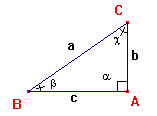
\includegraphics{img/triangoloretto.png} &
	\begin{tabular}{| p{4.5cm} | p{8.3cm} |}
		\nnt
		Cateto da ipotenusa & \texttt{$b = a \cdot \sin\beta = a \cdot \cos\gamma \ \ c = a \cdot \sin\gamma = a \cdot \cos\beta$} \nt
		Cateto da cateto & \texttt{$b = c \cdot \tan\beta = c \cdot \cot\gamma \ \ c = b \cdot \tan\gamma = b \cdot \cot\beta$} \nt
		Teorema dei seni & \texttt{$\dfrac{a}{\sin\alpha} = \dfrac{b}{\sin\beta} = \dfrac{c}{\sin\gamma}$} \nt
		Teorema del coseno & \texttt{$a^2 = b^2 + c^2 - 2bc\cos\alpha$}
		\tnn
	\end{tabular}
\end{tabular}



\subsection{Attrito}

\begin{tabular}{| p{9.5cm} | p{9.5cm} |}
\nnt
Forza risultante $(attrito\ statico)$ & \texttt{$F = \mu_s \cdot F_\perp$} \nt
Forza risultante $(attrito\ dinamico)$ & \texttt{$F = \mu_d \cdot F_hfi = \mu_d \cdot F_\perp$} \tnn
\end{tabular}

\subsection{Moto parabolico}

\begin{tabular}{| p{9.5cm} | p{9.5cm} |}
\nnt
Componenti del moto & 
	$\begin{cases}
	\texttt{$v_{0_x} = v_0 \cdot \cos\alpha$} \\
	\texttt{$v_{0_x} = v_0 \cdot \sin\alpha$} 
	\end{cases}$ \\[-5mm] \nt
Velocita & \texttt{$v = \sqrt{v_{0_x}^2 + v_{0_y}^2} \ \ \alpha = \arctan\dfrac{v_{0_y}}{v_{0_x}}$} \nt
Legge oraria & 
	$\begin{cases}
	\texttt{$x = x_0 + v_{0_x} \cdot t \ \ (moto\ rettilineo\ uniforme)$} \\
	\texttt{$y = -\dfrac12 \cdot g \cdot t^2 + v_{0_y} \cdot t + y_0 \ \ (moto\ uif.\ accelerato)$}
	\end{cases}$ \nt
Gittata & \texttt{$x_g = \dfrac{2 \cdot v_{0_x} \cdot v_{0_y}}{g}$} \nt
Gittata massima $(45^\circ,\ \dfrac\pi4)$ & \texttt{$x_{g_max} = \dfrac{v_0^2}{g}$} \nt
Tempo di volo & \texttt{$t_{volo} = \dfrac{2 \cdot v_{0_y}}{g}$} \nt
Altezza massima & \texttt{$y_{max} = \dfrac{v_{0_y}^2}{2 \cdot g}$} \nt
Tempo per raggiungere l'altezza massima & \texttt{$t_{y\ max} = \dfrac{v_{0_y}}{g}$} \tnn
\end{tabular}

\subsection{Leggi di Newton}

\begin{tabular}{| p{9.5cm} | p{9.5cm} |}
	\nnt
	I principio della dinamica & \texttt{$\sum_i\vec{F_i} = 0 \implies \vec{a} = 0$} \nt
	II principio della dinamica & \texttt{$\sum_i\vec{F_i} = m\vec{a}$} \nt
	III principio della dinamica & \texttt{$\vec{F}_{A\rightarrow B} = \vec{F}_{B\rightarrow A}$} \tnn
\end{tabular}

\subsection{Moto circolare uniforme}

\begin{tabular}{| p{9.5cm} | p{9.5cm} |}
	\nnt
	Frequenza e periodo & \texttt{$f = \dfrac{1}{t}$} \nt
	Legge oraria & \texttt{$\theta_t = \theta_0 + \omega \cdot t$} \nt
	Velocita tangenziale & \texttt{$v = \dfrac{s}{t}\ \ v = \dfrac{2\pi \cdot r}{t}$} \nt
	Velocita angolare & '\texttt{$\omega = \dfrac{2\pi}{t}\ \ v = \omega \cdot r$} \nt
	Accelerazione centripeta & \texttt{$a_c = \dfrac{v^2}{r}\ \ a_c = \omega^2 \cdot r$} \tnn
	
\end{tabular}

\subsection{Moto circolare uniformemente accelerato}

\begin{tabular}{| p{9.5cm} | p{9.5cm} |}
\nnt
Legge oraria $(t_i = 0)$ & \texttt{$\theta = \dfrac12 \cdot \alpha \cdot t^2 + \omega_0 \cdot t + \theta_0$} \nt
Accelerazione totale & \texttt{$\vec{a}_{tot} = \vec{a}_{tangenziale} + \vec{a}_{centripeta}$} \nt
Accelerazione angolare & \texttt{$\alpha = \dfrac{\omega_f - \omega_i}{t_f - t_i}$} \nt
Velocita angolare & \texttt{$\omega = \omega_0 + \alpha \cdot t$} \nt
Rapporto velocita - accelerazione & \texttt{$\omega^2 = \omega_0^2 + 2 \cdot \alpha \cdot (\theta - \theta_0)$} \nt
Forza centripeta & \texttt{$\vec{F}_c = m \cdot \vec{a}\ \ \vec{F}_c = m \cdot \dfrac{v^2}{r}\ \ \vec{F}_c = m \cdot \omega^2 \cdot r$} \tnn

\end{tabular}

\subsection{Forza elastica}

\begin{tabular}{| p{9.5cm} | p{9.5cm} |}
\nnt
Elongazione & \texttt{$\Delta x = L - (\pm L_0)$} \nt
Forza elastica $(Hooke's\ law)$ & \texttt{$\vec{F}_e = -k \cdot \vec{x}_{metri}$} \nt
Pulsazione & \texttt{$\omega = \sqrt{\dfrac{k}{m}}$} \nt
Periodo & \texttt{$T = \dfrac{2\pi}{\omega}$}
\tnn

\end{tabular}

\subsection{Lavoro}

\begin{tabular}{| p{9.5cm} | p{9.5cm} |}
\nnt
Lavoro & \texttt{$L = F \cdot \Delta s$} \nt
Energia cinetica & \texttt{$K = \dfrac12 \cdot m \cdot |\vec{v}|$} \nt
Energia potenziale & \texttt{$U = m \cdot g \cdot h$} \nt
Energia potenziale elastica & \texttt{$U_e = \dfrac12 \cdot k \cdot \Delta x^2$} \nt
Energia Meccanica $(totale)$ & \texttt{$M = K + U$} \nt
Principio di conservazione & \texttt{$\Delta M = M_f - M_0 = 0$} \tnn
\end{tabular}


\end{document}


\end{document}